


\documentclass[12pt, letterpaper, twoside]{article}
\usepackage[utf8]{inputenc}
\usepackage{tikz}
\usetikzlibrary{arrows, arrows.meta}
\usetikzlibrary{positioning}
\usepackage{verbatim}
\usepackage{amsmath}

\usepackage{siunitx}
\usepackage{xcolor}







 
\title{MPA Notes and Equations}
\author{Prof Don McGlinchey \thanks{Module Leader Mechanical Principles A}}
\date{October 2020}



\begin{document}
 
\maketitle

\bigskip

\begin{center}
	

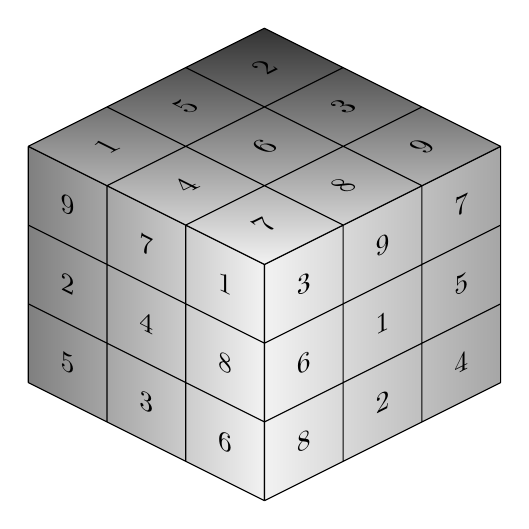
\begin{tikzpicture}[every node/.style={minimum size=1cm},on grid]

\begin{scope}[every node/.append style={yslant=-0.5},yslant=-0.5]
\shade[right color=gray!10, left color=black!50] (0,0) rectangle +(3,3);
\node at (0.5,2.5) {9};
\node at (1.5,2.5) {7};
\node at (2.5,2.5) {1};
\node at (0.5,1.5) {2};
\node at (1.5,1.5) {4};
\node at (2.5,1.5) {8};
\node at (0.5,0.5) {5};
\node at (1.5,0.5) {3};
\node at (2.5,0.5) {6};
\draw (0,0) grid (3,3);
\end{scope}
\begin{scope}[every node/.append style={yslant=0.5},yslant=0.5]
\shade[right color=gray!70,left color=gray!10] (3,-3) rectangle +(3,3);
\node at (3.5,-0.5) {3};
\node at (4.5,-0.5) {9};
\node at (5.5,-0.5) {7};
\node at (3.5,-1.5) {6};
\node at (4.5,-1.5) {1};
\node at (5.5,-1.5) {5};
\node at (3.5,-2.5) {8};
\node at (4.5,-2.5) {2};
\node at (5.5,-2.5) {4};
\draw (3,-3) grid (6,0);
\end{scope}
\begin{scope}[every node/.append style={
	yslant=0.5,xslant=-1},yslant=0.5,xslant=-1
]
\shade[bottom color=gray!10, top color=black!80] (6,3) rectangle +(-3,-3);
\node at (3.5,2.5) {1};
\node at (3.5,1.5) {4};
\node at (3.5,0.5) {7};
\node at (4.5,2.5) {5};
\node at (4.5,1.5) {6};
\node at (4.5,0.5) {8};
\node at (5.5,2.5) {2};
\node at (5.5,1.5) {3};
\node at (5.5,0.5) {9};
\draw (3,0) grid (6,3);
\end{scope}
\end{tikzpicture}
\end{center}

\newpage
 
Basic Concepts and Equations for Mechanical Principles A written with \LaTeX{} are Given in This Document!





\clearpage

\newpage

\section{Scalars and Vectors}

A \textbf{scalar} has only \textbf{magnitude}, that is, it can be fully described by a single number.
\linebreak 
\textit{Examples: Temperature, Distance, Speed, Mass.}

\bigskip    


A \textbf{vector} has both \textbf{magnitude and direction}, that is, as well as a number to quantify magnitude, we also need a way to indicate direction to describe a vector. 
\linebreak
\textit{Examples: Displacement, Velocity, Force, Momentum.}
\bigskip
We can describe the direction of a vector in several ways. \\ If the motion is only in one direction, for example, only along the x-axis and we take the usual convention of positive being to the right then we can say that a vector with a positive value (x +ve) has a direction to the right and a vector with a negative value (x -ve) has a direction to the left.\\  If the motion is in two directions we can; give the direction as an angle from the horizontal or indicate the direction by giving the vector's x and y components or by using unit vectors \textit{i} and \textit{j}.
$$ $$

\begin{tikzpicture}
%x-direction 1D
%arrow
\draw[<->, very thick, black] (1,-1) -- (10,-1);
%labels
\node [right] at (0,0) {$-ve$};
\node [right] at (10,0) {$+ve$};

\node [above] at (5,0.5) {$x-direction$};

\end{tikzpicture}
$$ $$
\textit{Figure 1} Indicating direction in one dimension, in this case the 'x-direction'.

\newpage

\begin{tikzpicture}

%axis and vector
\draw[<->, very thick, black] (1,-1) -- (9,-1);
\draw[<->, very thick, black] (5,-5) -- (5,3);
\draw[->, very thick, red] (5,-1) -- (8,2);

\draw[ultra thick, blue, ->] (6.5,-1) arc (0:65:1);

%labels
\node [right] at (0,-1) {$-x$};
\node [right] at (9,-1) {$+x$};
\node [right] at (5,-5) {$-y$};
\node [right] at (5,3) {$+y$};
\node [right, red] at (8,2) {$vector A$};
\node [right, blue] at (6.5,-0.5) {$angle\Theta_A$};

\end{tikzpicture}
$$ $$
\textit{Figure 2} Indicating direction in two dimensions, the magnitude of the vector is shown by the length of the line in red and the direction of the vector is indicated by the angle in blue.


The component form of vector A in two dimensions can be given using unit vectors as:
\begin{equation}
\overrightarrow{A} = A_x \hat{i} + A_y \hat{j}
\end{equation}




The Magnitude of vector A:
\begin{equation}
A = \sqrt{A_x^2 + A_y^2}
\end{equation}



The direction angle of vector A:

\begin{equation}
\Theta_A = tan^{-1} \left( \frac{A_y}{A_x} \right)
\end{equation}






\newpage

It is helpful to remember the trigonometry functions; sine, cosine and tangent when dealing with vectors and one way to help remember is the mnemonic SohCahToa:
$$ $$
\begin{tabular}{|c|c|c|c|}
	\hline 
	\rule[-1ex]{0pt}{2.5ex} Mnemonic & Trig function & Formula & Ratio \\ 
	\hline 
	\rule[-1ex]{0pt}{2.5ex} SOH & Sine & $sin\theta=\frac{O}{H}$ & Opposite over Hypotenuse \\ 
	\hline 
	\rule[-1ex]{0pt}{2.5ex} CAH & Cosine & $cos\theta=\frac{A}{H}$ & Adjacent over Hypotenuse \\ 
	\hline 
	\rule[-1ex]{0pt}{2.5ex} TOA & Tangent & $tan\theta=\frac{O}{A}$ & Opposite over Adjacent \\ 
	\hline 
\end{tabular} 


$$ $$

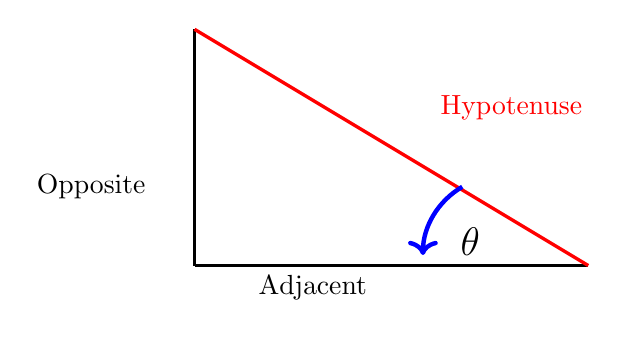
\begin{tikzpicture}

%trig
\draw[-, very thick, black] (3,0) -- (8,0);
\draw[-, very thick, black] (3,0) -- (3,3);
\draw[-, very thick, red] (3,3) -- (8,0);

\draw[ultra thick, blue, ->] (6.4,1) arc (120:180:1);

%labels
\node [below] at (4.5,0) {Adjacent};
\node [left] at (2.5,1) {Opposite};
\node [above] at (6.5,0) {\Large{$\theta$}};

\node [right, red] at (6.0,2) {Hypotenuse};


\end{tikzpicture}


$$ $$

In general when dealing with vectors [except when using the cross product] the problem can be tackled by:
\begin{enumerate}
	\item break the vectors into their x and y components
	\item separate and gather the x components and the y components 
	\item perform the operation or analysis separately for x and y components
	\item write the separate results for x and y components
	\item combine these x and y results together using vector addition  
\end{enumerate}

\bigskip

The following diagram might also help in selecting the correct angles.
\bigskip

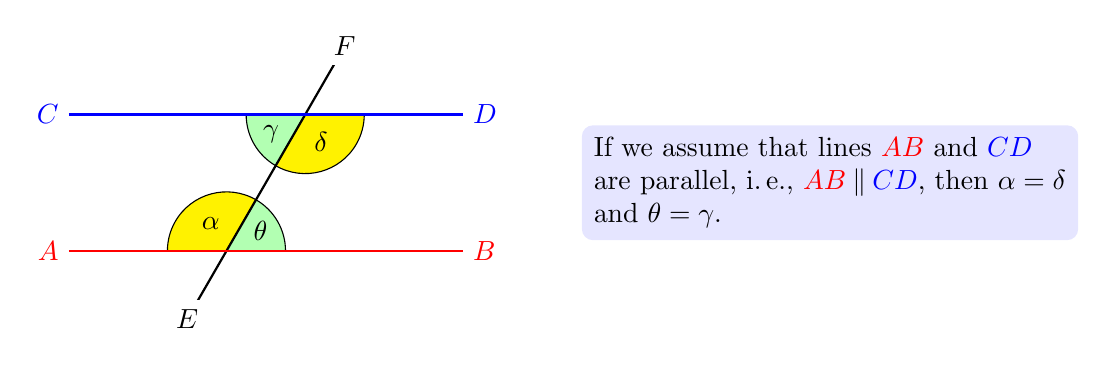
\begin{tikzpicture}
\draw[fill=yellow] (0,0) -- (60:.75cm) arc (60:180:.75cm);
\draw(120:0.4cm) node {$\alpha$};

\draw[fill=green!30] (0,0) -- (right:.75cm) arc (0:60:.75cm);
\draw(30:0.5cm) node {$\theta$};

\begin{scope}[shift={(60:2cm)}]
\draw[fill=green!30] (0,0) -- (180:.75cm) arc (180:240:.75cm);
\draw (30:-0.5cm) node {$\gamma$};

\draw[fill=yellow] (0,0) -- (240:.75cm) arc (240:360:.75cm);
\draw (-60:0.4cm) node {$\delta$};
\end{scope}

\begin{scope}[thick]
\draw (60:-1cm) node[fill=white] {$E$} -- (60:3cm) node[fill=white] {$F$};
\draw[red]                   (-2,0) node[left] {$A$} -- (3,0) 
node[right]{$B$};
\draw[blue,shift={(60:2cm)}] (-3,0) node[left] {$C$} -- (2,0) 
node[right]{$D$};

\draw[shift={(60:1cm)},xshift=4cm]
node [right,text width=6cm,rounded corners,fill=blue!10,inner sep=1ex]
{
	If we assume that lines $\color{red}AB$ and $\color{blue}CD$ are
	parallel, i.\,e., ${\color{red}AB} \mathbin{\|} \color{blue}CD$,
	then $\alpha = \delta$ and $\theta = \gamma$.
};
\end{scope}
\end{tikzpicture}



\newpage

\section{MOTION ALONG A STRAIGHT LINE}

\bigskip

We can in many cases approximate an objects motion in space as being along a straight line.  In which case we can determine aspects of its motion such as displacement, velocity and acceleration using relatively simple equations.
 \bigskip
 
\emph{Displacement} $\Delta x$ is the change in position of an object from its initial position to its final position.  
\begin{align}
\Delta x = x_f - x_i
\end{align}



If an object moves in a number of individual 'steps' then we can calculate its \emph{Total Displacement}
\begin{equation}
\Delta x_{Total} = \Sigma \Delta x_i
\end{equation}

If an object moves from position $x_1$ at a time $t_1$ to a new position $x_2$ at a time $t_2$ we can determine its \emph{Average Velocity}
\begin{equation}
\bar{v} = \frac{\Delta x}{\Delta t} = \frac{x_2 - x_1}{t_2 - t_1}
\end{equation}


Unless the motion is with constant velocity is  will be  different from the velocity at any particular instance in time, that is the \emph{Instantaneous Velocity}
\begin{equation}
v(t) = \frac{dx(t)}{dt}
\end{equation}


In a very similar way we can determine\emph{ Average Acceleration}
\begin{equation}
\bar{a} = \frac{\Delta v}{\Delta t} = \frac{v_2 - v_1}{t_2 - t_1}
\end{equation}

and \emph{Instantaneous Acceleration}
\begin{equation}
a(t) = \frac{dv(t)}{dt}
\end{equation}


\bigskip
If the motion is with \textbf{\emph{constant acceleration}} then we can use a set of equations known as the kinematic equations.
\bigskip

Velocity from Acceleration
\begin{equation}
v = v_0 + at
\end{equation}


Position from velocity and acceleration
\begin{equation}
x = x_0 + v_0 + \frac{1}{2} a t^2
\end{equation} 


Velocity from distance 
\begin{equation}
v^2 = v_0^2 + 2a(x - x_0)
\end{equation}


\bigskip

When considering object falling under the effect of gravity, that is with constant acceleration $-g$ where $g=9.8m/s^2$, then a very similar set of equations can be used replacing $a$ with $-g$, for example;

Height of free fall from starting position $y_0$ and initial velocity $v_0$
\begin{equation}
y = y_0 + v_0 t - \frac{1}{2} g t^2
\end{equation}


\newpage

\section{MOTION IN TWO AND THREE DIMENSIONS}
\bigskip

The position of a object in 3D space can be described by its \emph{Position Vector}
\begin{equation}
\overrightarrow{r}(t) = x(t) \hat{i} + y(t) \hat{j} + z(t) \hat{k}
\end{equation}


\bigskip

Consider then a movement of an object from a position at $t_1$ to a new position at time $t_2$, the displacement of that object can be determined by the vector addition of the two position vectors, giving the \emph{Displacement Vector}
\begin{equation}
\Delta \overrightarrow{r}=\overrightarrow{r}(t_2) -  \overrightarrow{r}(t_1)
\end{equation}

\bigskip
and the \emph{Average Velocity} can be found from;
\begin{equation}
\overrightarrow{v_{avg}} = \frac{\overrightarrow{r}(t_2) -  \overrightarrow{r}(t_1)}{t_2 - t_1}
\end{equation}


As with motion in 1D the \emph{Instantaneous Velocity Vector} in 3D is 
\begin{equation}
\overrightarrow{v}(t)= \frac{d \overrightarrow{r}}{dt}
\end{equation}


\bigskip
As with other vectors we can write the Velocity in terms of components;
\begin{equation}
\overrightarrow{v}(t) = v_x(t) \hat{i} + v_y(t) \hat{j} + v_z(t) \hat{k}
\end{equation}


This approach is very useful in problem solving where each [\textit{orthogonal}] component x, y and z can be treated independently and only re-combined at the end to give a final result.  If acceleration is constant then we can use the kinematic equations independently in each component direction. 

\bigskip

Where\emph{Instantaneous Acceleration}
\begin{equation}
\overrightarrow{a}(t)= \frac{d \overrightarrow{v}(t)}{dt}
\end{equation}







\newpage

\section{NEWTON'S LAWS OF MOTION}

The study of how forces affect the motion of objects is known as \emph{dynamics}, up to now we have restricted the study to equations the motion or \emph{kinematic equations}.  The most important relationships and equations in this section are based on \textbf{Newton's Laws of Motion} and to aid solve problems we will use \emph{free body diagrams}. 
\bigskip
In many problems we can treat the mass of a real object as acting at a point [centre of mass] and the forces acting on the object as force vectors acting on that point.  This forms the basis of drawing free body diagrams.
\bigskip



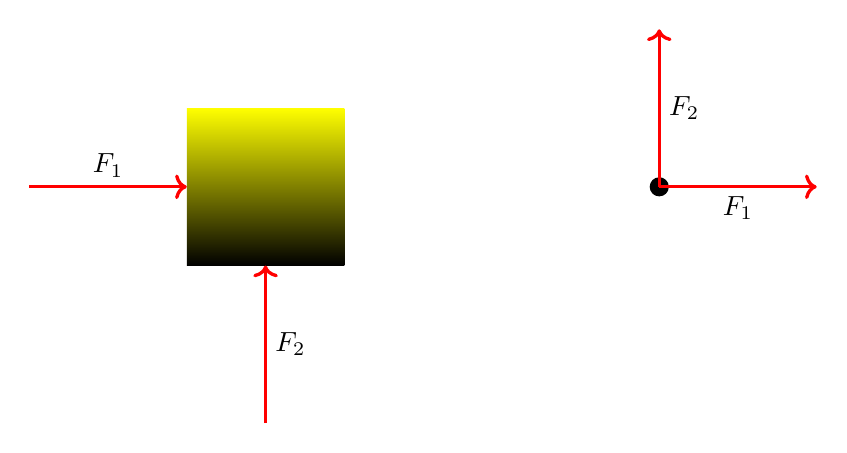
\begin{tikzpicture}

%box
\shade[top color=yellow, bottom color=black] (2,0) rectangle (4,2);
\draw [->, very thick, red] (0,1) -- (2,1);
\draw [->, very thick, red] (3,-2) -- (3,0);

%dot
\filldraw[color=black, fill=black, very thick](8,1) circle (0.1);
\draw [->, very thick, red] (8,1) -- (10,1);
\draw [->, very thick, red] (8,1) -- (8,3);


%labels
\node [above] at (1,1) {$F_1$};
\node [right] at (3,-1) {$F_2$};
\node [right] at (8,2) {$F_2$};
\node [below] at (9,1) {$F_1$};

\end{tikzpicture}

\bigskip
\emph{Figure 3} Two forces $\overrightarrow{F}_1$ and $\overrightarrow{F}_2$ acting on a box and the representation as a free body diagram.  

\bigskip 

This is a very simple case but we can use free body diagrams in more complex problems to help to visualise the magnitudes and directions of the forces acting on a body.  Once this is clear we can calculate the \emph{Net External Force}:
\begin{equation}
\overrightarrow{F}_{net} = \Sigma \overrightarrow{F} = \overrightarrow{F}_1+\overrightarrow{F}_2 +...
\end{equation}

\bigskip
\textbf{Problem-Solving Strategy: Drawing Free-Body Diagrams}
\begin{enumerate}
	\item Draw the object under consideration. If you are treating the object as a particle, represent the object as a point. Place this point at the origin of an xy-coordinate system.
	\item Include all forces that act on the object, representing these forces as vectors. However, do not include the net force on the object or the forces that the object exerts on its environment.
	\item Resolve all force vectors into x- and y-components.
	\item Draw a separate free-body diagram for each object in the problem.
\end{enumerate}

\bigskip

\textbf{Newton’s First Law of Motion}\\
\texttt{\textcolor{blue}{A body at rest remains at rest or, if in motion, remains in motion at constant velocity unless acted on by a net external force.}}

\bigskip
We can write Newton's First Law more mathematically
\begin{equation}
\overrightarrow{v} = \textnormal{constant when} \overrightarrow{F}_{net} = \overrightarrow{0} N
\end{equation}

\bigskip
\textbf{Newton’s Second Law of Motion}\\
\texttt{\textcolor{blue}{The acceleration of a system is directly proportional to and in the same direction as the net external force acting on the system and is inversely proportional to its mass}}

\bigskip

This can be written in equation form as:

\begin{equation}
\overrightarrow{a} = \frac{\overrightarrow{F}_{net}}{m}
\end{equation}

\bigskip

It is more usual to see Newton's Second Law, written in \emph{Vector Form} as:


\begin{equation}
\overrightarrow{F}_{net} = \Sigma \overrightarrow{F} = m \overrightarrow{a}
\end{equation}




\bigskip

We can also write Newton's Second Law in \emph{Component Form}, where we treat the x,y and z components separately:

\begin{equation}
\Sigma \overrightarrow{F}_x = m \overrightarrow{a_x},\;\; \Sigma \overrightarrow{F}_y = m \overrightarrow{a_y}, \;\;\Sigma \overrightarrow{F}_z = m \overrightarrow{a_z}
\end{equation}


\bigskip

By recognising that acceleration $a$ can be written as $\frac{dv}{dt}$ and momentum $p = mv$, we can write Newton's Second Law in \emph{Momentum Form} 

\begin{equation}
\overrightarrow{F}_{net} = \frac{d \overrightarrow{p}}{dt}
\end{equation}

\bigskip

That is, another way of expressing Newton's Second Law is that the net force acting on an object is equal to the rate of change of momentum of that object. 


\bigskip

Newton's Second Law is used in our definition of \textbf{weight}, where in Vector Form, the\emph{ Definition of Weight} can be given as:
\begin{equation}
\overrightarrow{w} = m \overrightarrow{g}
\end{equation} 

\bigskip

Or simply in Scalar Form:

\begin{equation}
w = mg
\end{equation}

\bigskip

An important thing to notice here is that \underline{weight is a force} and will have SI units [N].

\bigskip


\bigskip
\textbf{Newton’s Third Law of Motion}\\
\texttt{\textcolor{blue}{Whenever one body exerts a force on a second body, the first body experiences a force that is equal in magnitude and opposite in direction to the force that it exerts}}

\bigskip

This can be written in equation form as:

\begin{equation}
\overrightarrow{F}_{AB} = - \overrightarrow{F}_{BA}
\end{equation}


\bigskip

Newton’s Third Law of Motion is used commonly in the following:

\bigskip


Normal force on an object resting on a horizontal surface,
vector form.
\begin{equation}
\overrightarrow{N} = -m \overrightarrow{g}
\end{equation}

Normal force on an object resting on a horizontal surface,
scalar form.
\begin{equation}
N = -mg
\end{equation}


Normal force on an object resting on an inclined surface $\theta$ from the horizontal, in
scalar form.

\begin{equation}
N = -m g cos \theta
\end{equation}

\newpage


\section{APPLICATION OF NEWTON'S LAWS}

\bigskip

When applying Newton's Laws to solving problems it is useful to follow a consistent strategy or process.

 
\bigskip
\textbf{Problem-Solving Strategy: Applying Newton’s Laws of Motion}
\begin{enumerate}
	\item Identify the mechanical principles involved; list the information and values given and the unknowns to be calculated.
	\item Sketch the problem, using arrows to represent all forces.
	\item Determine the "system of interest". Represent this in a free-body diagram with component x, y and z forces. 
	\item Apply Newton’s second law to solve the problem in component form. (If necessary, apply appropriate kinematic equations for motion along a straight line).
	\item Treat as vectors to get a result.
	\item Check that the solution is reasonable.
\end{enumerate}

\bigskip

In these problems we may also have to deal with the forces associated with some form of resistance or friction which opposes the motion.  The two most common are friction between two surfaces and the resistance due to motion through a fluid [drag].

\bigskip






Magnitude of static friction
\begin{equation}
f_s \leq \mu_s N
\end{equation}



Magnitude of kinetic friction
\begin{equation}
f_k \leq \mu_k N
\end{equation}



Drag Force
\begin{equation}
F_D=\frac{1}{2} C_D \rho A v^2 
\end{equation}


Stokes' Law
\begin{equation}
F_s = 6 \pi r \eta v
\end{equation}



\bigskip

A body undergoing \textbf{Uniform Circular Motion} will experience \emph{Centripetal Force}
\begin{equation}
F_c = m \frac{v^2}{r} = mr\omega^2
\end{equation}

\bigskip
\begin{center}


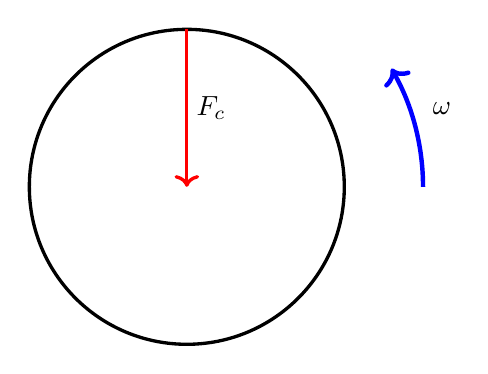
\begin{tikzpicture}
\centering
%circle
\draw [black, very thick](1,1) circle (2.0);
\draw [ultra thick, blue, ->] (4,1) arc (0:30:3);
\draw [->, very thick, red] (1,3) -- (1,1);


%labels

\node [right] at (1,2) {$F_c$};
\node [right] at (4,2) {$\omega$};

\end{tikzpicture}
\end{center}


\bigskip
where $\omega$ is the \emph{angular velocity} and $r$ is the \emph{radius of motion}
\begin{equation}
\omega = \frac{\Delta \theta}{\delta t}
\end{equation}







\newpage


\section{WORK AND KINETIC ENERGY}

\bigskip

The work done on a system by a constant force is the product of the component of the force in the direction of motion times the distance through which the force acts. 

\bigskip


Work Done by a constant force in line with displacement
\begin{equation}
W = F \cdot d
\end{equation}

\begin{equation}
W = Fd\cos \theta
\end{equation}

\bigskip

We can show this graphically.

\bigskip


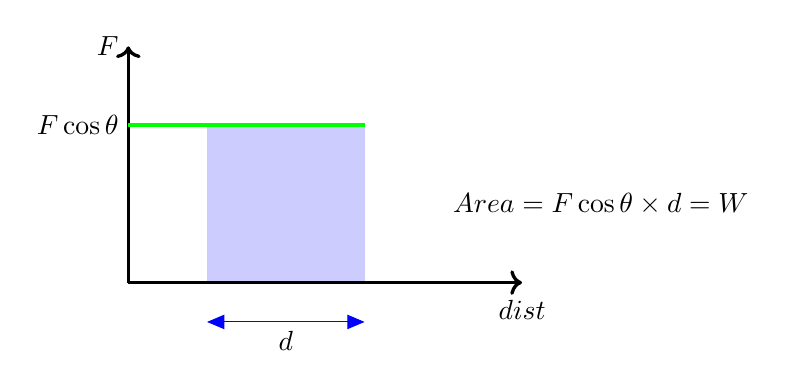
\begin{tikzpicture}

%box
\filldraw[color=blue!20] (1,0) rectangle (3,2);

%axis

\draw [->, very thick] (0,0) -- (0,3);
\draw [->, very thick] (0,0) -- (5,0);

%lines
\draw[very thick, green] (0,2) -- (3,2);
\draw[>=triangle 45, <->, blue] (1,-0.5) -- (3,-0.5);

%labels
\node [left] at (0,2) {$F\cos \theta$};
\node [below] at (5,-0.1) {$dist$};
\node [left] at (0,3) {$F$};
\node [below] at (2,-0.5) {$d$};

\node [right] at (4,1) {$Area = F \cos \theta \times d = W$};

\end{tikzpicture}


\bigskip


If the force is not constant and or the path from A to B is not linear we can use the Work done by a force over an infinitesimal displacement;

\begin{equation}
dW = \overrightarrow{F} \cdot d \overrightarrow{r} = | \overrightarrow{F} | | d \overrightarrow{r} | \cos \theta
\end{equation}

\bigskip

and then calculate the Work done by a force acting along a path from A to B;

\begin{equation}
W_{AB} = \int\limits_A^B \overrightarrow{F} \cdot d \overrightarrow{r}
\end{equation}

\bigskip

If an object is lifted straight up from A to B against Earth's gravity near its surface at constant speed, then the force needed to lift it is equal to its weight  $mg$ . The Work done going from A to B by Earth's gravity near its surface is then;

\begin{equation}
W_{grav,AB} = -mg(y_B - y_A)
\end{equation}

\bigskip

If we take the datum $y_A = 0$ and $y_B$ is then some height $h$ above the datum, we can make two related statements.
One, the work done in raising the object of mass $m$ to a height $h$ is:
\begin{equation}
W = -mgh
\end{equation}

\bigskip

and the gain in \emph{Potential Energy} is:
\begin{equation}
PE = mgh
\end{equation}


\bigskip

In a similar manner the work done going from A to B by one-dimensional spring force is:
\begin{equation}
W_{spring,AB} = - \frac{1}{2} k (x_B^2 - x_A^2)
\end{equation}
\bigskip

and the gain in potential energy of the spring is:

\begin{equation}
PE_{spring,AB} =  \frac{1}{2} k (x_B^2 - x_A^2)
\end{equation}
\bigskip

\bigskip

The energy associated with a moving object is called \emph{kinetic energy}.  The translational kinetic energy (KE) of a mass  $m$  moving at a speed  $v$ . (Translational kinetic energy is distinct from rotational kinetic energy, which is considered later) can be written as:

\begin{equation}
KE = \frac{1}{2} m v^2
\end{equation}

\bigskip 


The kinetic energy of an object can be related to its momentum


\begin{equation}
KE = \frac{1}{2} m v^2 = \frac{p^2}{2m}
\end{equation}

\bigskip


The \emph{Work-Energy Theorem} states that the net work on a system equals the change in its KE.

\begin{equation}
W_{net} = \frac{1}{2}m V^2
\end{equation}

\bigskip

We can also define here Power as a rate of doing work:
\begin{equation}
P = \frac{dW}{dt}
\end{equation}
\bigskip

and Power as the dot product of force and velocity:
\begin{equation}
P = \overrightarrow{F} \cdot \overrightarrow{v} 
\end{equation}


\newpage


\section{LINEAR MOMENTUM AND COLLISIONS}

\bigskip


Linear momentum is defined as the product of a system’s mass multiplied by its velocity:
\begin{equation}
\overrightarrow{p} = m \overrightarrow{v}
\end{equation}

\bigskip
Newton's second law of motion can also be written in terms of momentum, where the net external force $F_{net}$ equals the change in momentum $\Delta p$ of a system divided by the time taken for the change $\Delta t$.

\begin{equation}
F_{net} = \frac {\Delta p}{\Delta t}
\end{equation}

\bigskip

We can rearrange this to give:

\begin{equation}
\Delta p = F_{net}{\Delta t}
\end{equation}

\bigskip
The term $F_{net}{\Delta t}$ is know as \emph{impulse} and is often given the symbol $J$.  


\bigskip

In vector notation Impulse could be written as:

\begin{equation}
\overrightarrow{J} = \int\limits_{t_i}^{t_f} \overrightarrow{F}(t) dt  = \overrightarrow{J} = \overrightarrow{F}_{ave} \Delta t 
\end{equation}

\bigskip

and the Impulse-momentum theorem would then be written as:

\begin{equation}
\overrightarrow{J} = \Delta \overrightarrow{p}
\end{equation}
 \bigskip
 
we can then write the Average force from momentum as:
\begin{equation}
\overrightarrow{F} (t) = \frac{d \overrightarrow{p}}{dt}
\end{equation}

\bigskip

An important property of momentum is that it is \emph{conserved} in an isolated system.  So we can write a Generalised conservation of momentum.

\begin{equation}
\displaystyle\sum_{j=1}^{N} \overrightarrow{p}_j = constant
\end{equation}

\bigskip

An isolated system is defined to be one for which the net external force is zero  ($F_{net.ext}=0$), where:

\begin{equation}
\overrightarrow{F}_{net.ext} = \displaystyle\sum_{j=1}^{N} \frac{d \overrightarrow{p}_j}{dt}
\end{equation}


\bigskip

This fact that momentum is conserved allows us to use this in the study of collisions.  We will look at two basic types of collision 
\begin{enumerate}
	\item elastic collisions
	\item non-elastic collisions 
\end{enumerate} 

\bigskip

Beginning with elastic collisions we can define a elastic collision as one that conserves internal kinetic energy. If we consider two objects in an elastic collision with initial momentum $p_1$ and $p_2$ and final momentum $p'_1$ and $p'_2$ then the conservation of momentum means:

\begin{equation}
p_1 + p_2 = p'_1 + p'_2 
\end{equation}

or \\
\begin{equation}
m_1 v_1 + m_2 v_2 = m_1 v'_1 + m_2 v'_2
\end{equation}
\bigskip

and because in an elastic collision internal kinetic energy is conserved

\begin{equation}
\frac{1}{2} m_1 v^2_1 + \frac{1}{2} m_2 v^2_2 = \frac{1}{2} m_1 v'^2_1 + \frac{1}{2} m_2 v'^2_2
\end{equation}

\bigskip


% elastic collision before
\textbf{BEFORE}

\begin{center}
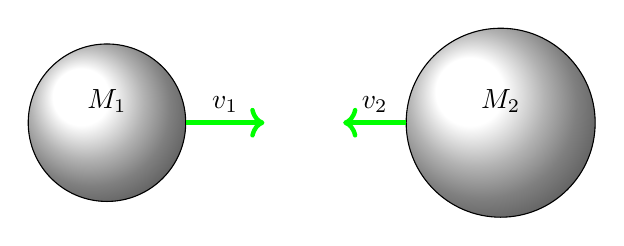
\begin{tikzpicture} % "THE GLOBE" showcase

%spherical objects
\filldraw[ball color=white] (0,0) circle (1.0);
\filldraw[ball color=white] (5,0) circle (1.2);

%arrows
\draw[->, ultra thick, green] (1,0) -- (2,0);
\draw[->, ultra thick, green] (3.8,0) -- (3,0);

%labels
\node[above] at (0,0) {$M_1$};
\node[above] at (5,0) {$M_2$};

\node[above] at (1.5,0) {$v_1$};
\node[above] at (3.4,0) {$v_2$};


\end{tikzpicture}
\end{center}


\bigskip

% elastic collision after
\textbf{AFTER}

\begin{center}
	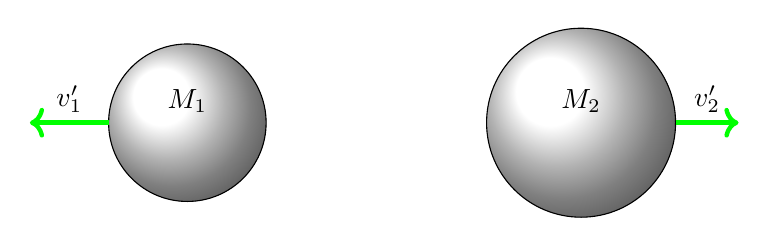
\begin{tikzpicture} % "THE GLOBE" showcase
	
	%spherical objects
	\filldraw[ball color=white] (0,0) circle (1.0);
	\filldraw[ball color=white] (5,0) circle (1.2);
	
	%arrows
	\draw[->, ultra thick, green] (-1,0) -- (-2,0);
	\draw[->, ultra thick, green] (6.2,0) -- (7,0);
	
	%labels
	\node[above] at (0,0) {$M_1$};
	\node[above] at (5,0) {$M_2$};
	
	\node[above] at (-1.5,0) {$v'_1$};
	\node[above] at (6.6,0) {$v'_2$};
	
	
	\end{tikzpicture}
\end{center}






\bigskip








An \textbf{\emph{inelastic}} collision is one in which the internal kinetic energy changes (it is \emph{not} conserved). A collision in which the objects stick together is sometimes called “perfectly inelastic.”

\bigskip

\begin{equation}
m_1 v_1 + m_2 v_2 = (m_1  + m_2) v_3
\end{equation}




\bigskip

% inelastic collision before
\textbf{BEFORE}

\begin{center}
	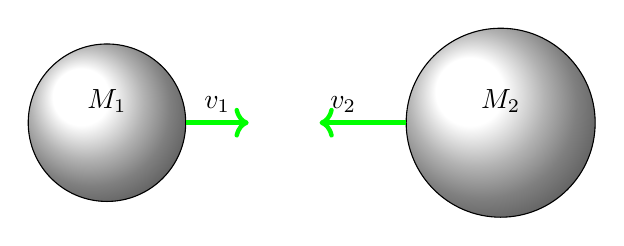
\begin{tikzpicture} % "THE GLOBE" showcase
	
	%spherical objects
	\filldraw[ball color=white] (0,0) circle (1.0);
	\filldraw[ball color=white] (5,0) circle (1.2);
	
	%arrows
	\draw[->, ultra thick, green] (1,0) -- (1.8,0);
	\draw[->, ultra thick, green] (3.8,0) -- (2.7,0);
	
	%labels
	\node[above] at (0,0) {$M_1$};
	\node[above] at (5,0) {$M_2$};
	
	\node[above] at (1.4,0) {$v_1$};
	\node[above] at (3.0,0) {$v_2$};
	
	
	\end{tikzpicture}
\end{center}


\bigskip

% inelastic collision after
\textbf{AFTER}

\begin{center}
	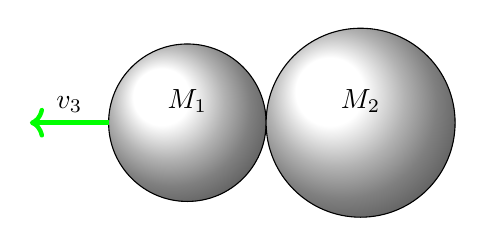
\begin{tikzpicture} % "THE GLOBE" showcase
	
	%spherical objects
	\filldraw[ball color=white] (0,0) circle (1.0);
	\filldraw[ball color=white] (2.2,0) circle (1.2);
	
	%arrows
	\draw[->, ultra thick, green] (-1,0) -- (-2,0);

	
	%labels
	\node[above] at (0,0) {$M_1$};
	\node[above] at (2.2,0) {$M_2$};
	
	\node[above] at (-1.5,0) {$v_3$};
	
	
	
	\end{tikzpicture}
\end{center}


\bigskip

\textbf{\emph{Collisions in 2D}} can be analysed using vectors and by treating the $x$-components and the $y$-components independently.  For example for an ellastic collision.

\begin{equation}
p_{x1} + p_{x2} = p'_{x1} + p'_{x2}
\end{equation}

and \\
\begin{equation}
p_{y1} + p_{y2} = p'_{y1} + p'_{y2}
\end{equation}




\bigskip



\newpage


\section{FIXED AXIS ROTATION}
\bigskip




The \emph{Angular Position} $\theta$ of an object rotating at a radius $r$ which is displaced through an arc length $s$ is given by:

\begin{equation}
\theta = \frac{s}{r}
\end{equation} 
\bigskip
 
\begin{center}
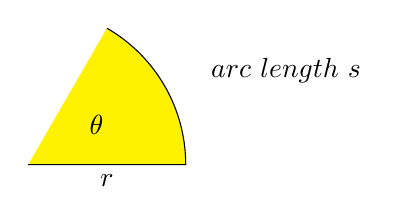
\begin{tikzpicture}
\draw[fill=yellow] (0,0) -- (00:2.0cm) arc (0:60:2.0cm);
\draw(30:1.0cm) node {$\theta$};
\node [right] at (2.2,1.2) {$arc \ length \ s$};
\node [below] at (1.0, 0.0) {$r$};

\end{tikzpicture}
\end{center}
\bigskip

As shown earlier for uniform circular motion, [which is motion in a circle at constant speed and, hence, constant angular velocity] \emph{angular velocity}  $\omega$  was defined as the time rate of change of angle $\theta$ :
Angular Velocity:
\begin{equation}
\omega = \frac{d \theta}{dt}
\end{equation}


\bigskip

The \emph{Tangential Velocity} $v_t$ is then 

\begin{equation}
v_t = r \omega
\end{equation}



\bigskip

\begin{center}
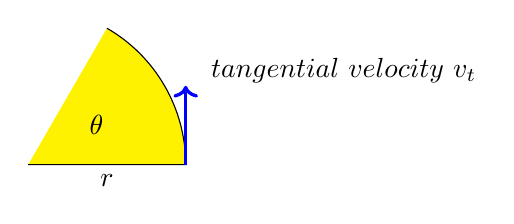
\begin{tikzpicture}
	\draw[fill=yellow] (0,0) -- (00:2.0cm) arc (0:60:2.0cm);
	\draw(30:1.0cm) node {$\theta$};
	\node [right] at (2.2,1.2) {$tangential \ velocity \ v_t$};
	\draw [->, blue, very thick ]  (2.0, 0.0) -- (2.0, 1.0);
	\node [below] at (1.0, 0.0) {$r$};
\end{tikzpicture}
\end{center}
\bigskip


In a similar way we can write equations for \emph{Angular Acceleration}
\begin{equation}
\alpha =\frac{d \omega}{dt} = \frac{d^2 \theta}{d t^2}.
\end{equation}


 and \emph{Tangential Acceleration}

\begin{equation}
a_t = r \alpha
\end{equation}


\bigskip

The Kinematics for rotational motion is completely analogous to translational kinematics, where:

Angular Displacement
\begin{equation}
\theta_f = \theta_0 + \bar{\omega} t
\end{equation}



Angular velocity with constant acceleration
\begin{equation}
\omega_f = \omega_0 + \alpha t
\end{equation}



Angular displacement with constant acceleration
\begin{equation}
\theta_f = \theta_0 + \omega_0 t + \frac{1}{2} \alpha t^2 
\end{equation}

\bigskip



Moment of Inertia
$$ I = \sum_j m_j r_j^2 $$


Rotational Kinetic Energy
$$ K = \frac{1}{2} I \omega^2 $$


Torque Vector
$$ \overrightarrow{\tau} = \overrightarrow{r} \times \overrightarrow{F}$$



Newton's 2nd Law of Rotation
$$ \sum_i \tau_i = I \alpha $$



Rotational Power
$$ P = \tau \omega $$




\newpage









Percentage Uncertainty 
$$=\frac{\delta A}{A} \times 100\%$$

\vfil


\textbf{VECTORS}
$$  $$

Multiplication by a scalar
$$\overrightarrow{B}=\alpha \overrightarrow{A}$$


Cummutative Law
$$\overrightarrow{A} +\overrightarrow{B} = \overrightarrow{B} + \overrightarrow{A}$$ 


Associative Law
$$(\overrightarrow{A} + \overrightarrow{B}) + \overrightarrow{C} = \overrightarrow{A} + (\overrightarrow{B} + \overrightarrow{C})$$



The component form of a vector in two dimensions
$$\overrightarrow{A} = A_x \hat{i} + A_y \hat{j}$$




The Magnitude of a vector in a plane
$$A = \sqrt{A_x^2 + A_y^2}$$



The direction angle of a vector in a plane
$$\Theta_A = tan^{-1} \left( \frac{A_y}{A_x} \right)$$




The component form of a vector in three dimensions
$$\overrightarrow{A} = A_x \hat{i} + A_y \hat{j} + A_z \hat{k}$$


The Magnitude of a vector in three dimensions
$$A = \sqrt{A_x^2 + A_y^2 + A_z^2}$$



Definition of the \textbf{Scalar} product
$$\overrightarrow{A} . \overrightarrow{B}= AB \cos \theta$$


Scalar product in terms of the scalar components of vectors
$$\overrightarrow{A} . \overrightarrow{B}= A_x B_x + A_y B_y + A_z B_z$$



Dot products odf unit vectors
$$\hat{i} . \hat{j} = \hat{j} . \hat{k} = \hat{k} . \hat{i} = 0$$



Magnitude of the \textbf{vector} product
$$\mid \overrightarrow{A} \times \overrightarrow{B} \mid= AB \sin \theta$$



Cross products of unit vectors
$$\hat{i} \times \hat{j} =+ \hat{k}, \hat{j} \times \hat{k} = +\hat{i}, \hat{k} \times \hat{i} =+ \hat{j}$$
 



The Cross product in terms of scalar components of vectors
$$\overrightarrow{A} \times \overrightarrow{B} = (A_y B_z - A_z B_y) \hat{i} + (A_z B_x - A_x B_z) \hat{j} + (A_x B_y - A_y B_x) \hat{k}$$



\newpage

MOTION ALONG A STRAIGHT LINE
$$ $$



Displacement
$$\Delta x = x_f - x_i$$


Total Displacement
$$\Delta x_{Total} = \Sigma \Delta x_i$$

Average Velocity
$$\bar{v} = \frac{\Delta x}{\Delta t} = \frac{x_2 - x_1}{t_2 - t_1}$$

Instantaneous Velocity
$$v(t) = \frac{dx(t)}{dt}$$

Average Acceleration
$$\bar{a} = \frac{\Delta v}{\Delta t} = \frac{v_2 - v_1}{t_2 - t_1}$$

Instantaneous Acceleration
$$a(t) = \frac{dv(t)}{dt}$$

Velocity from Acceleration [constant a]
$$v = v_0 + at$$

Position from velocity and acceleration [constant a]
$$x = x_0 + v_0 + \frac{1}{2} a t^2$$

Velocity from distance [constant a]
$$v^2 = v_0^2 + 2a(x - x_0)$$

Height of free fall
$$y = y_0 + v_0 t - \frac{1}{2} g t^2$$


\newpage

MOTION IN TWO AND THREE DIMENSIONS

$$ $$  

Position Vector
$$\overrightarrow{r}(t) = x(t) \hat{i} + y(t) \hat{j} + z(t) \hat{k}$$


Displacement Vector
$$\Delta \overrightarrow{r}=\overrightarrow{r}(t_2) -  \overrightarrow{r}(t_1)$$


Velocity Vector
$$\overrightarrow{v}(t)= \frac{d \overrightarrow{r}}{dt}$$


Velocity in Terms of Components
$$\overrightarrow{v}(t) = v_x(t) \hat{i} + v_y(t) \hat{j} + v_z(t) \hat{k}$$


Average Velicity
$$\overrightarrow{v}_avg = \frac{\overrightarrow{r}(t_2) -  \overrightarrow{r}(t_1)}{t_2 - t_1}$$


Instantanious Acceleration
$$\overrightarrow{a}(t)= \frac{d \overrightarrow{v}(t)}{dt}$$


Centripetal Acceleration
$$a_c = \frac{v^2}{r}$$



\newpage

NEWTON'S LAWS OF MOTION

$$ $$


Net External Force
$$\overrightarrow{F}_{net} = \Sigma \overrightarrow{F} = \overrightarrow{F}_1+\overrightarrow{F}_2 +...$$


Newton's First Law
$$\overrightarrow{v} = constant when \overrightarrow{F}_{net} = \overrightarrow{0} N$$


Newton's Second Law, Vector Form
$$\overrightarrow{F}_{net} = \Sigma \overrightarrow{F} = m \overrightarrow{a}$$


Newton's Second Law, Component Form
$$\Sigma \overrightarrow{F}_x = m \overrightarrow{a_x}, \Sigma \overrightarrow{F}_y = m \overrightarrow{a_y},\Sigma \overrightarrow{F}_z = m \overrightarrow{a_z}$$



Newton's Second Law, Momentum Form
$$\overrightarrow{F}_{net} = \frac{d \overrightarrow{p}}{dt}$$


Defination of Weight, Vector Form
$$\overrightarrow{w} = m \overrightarrow{g}$$


Defination of Weight, Vector Form
$$w = mg$$


Newton's Thrid Law
$$\overrightarrow{F}_{AB} = - \overrightarrow{F}_{BA}$$

Normal force on an object resting on a horizontal surface,
vector form.
$$\overrightarrow{N} = -m \overrightarrow{g}$$

Normal force on an object resting on a horizontal surface,
scalar form.
$$N = -mg$$

Normal force on an object resting on an inclined surface,
scalar form.
$$N = -m g cos \theta$$



\newpage

APPLICATION OF NEWTON'S LAWS

$$ $$

Magnitude of static friction
$$f_s \leq \mu_s N$$


Magnitude of kinetic friction
$$f_k \leq \mu_k N$$


Centripetal Force
$$F_c = m \frac{v^2}{r} = mr\omega^2$$



Drag Force
$$F_D=\frac{1}{2} C_D \rho A v^2 $$


Stokes' Law
$$F_s = 6 \pi r \eta v $$








\newpage

WORK AND KINETIC ENERGY

$$ $$


Work Done by a force in line with displacement
$$ W = F \cdot d $$


Work done by a force over an infinitesimal displacement
$$ dW = \overrightarrow{F} \cdot d \overrightarrow{r} = | \overrightarrow{F} | | d \overrightarrow{r} | \cos \theta $$


Work done by a force acting along a path from A to B
$$ W_{AB} = \int\limits_A^B \overrightarrow{F} \cdot d \overrightarrow{r} $$


Work done going from A to B by Earth's gravity near its surface
$$ W_{grav,AB} = -mg(y_B - y_A) $$


Work done going from A to B byone-dimensional spring force
$$ W_{spring,AB} = - \frac{1}{2} k (x_B^2 - x_A^2) $$
%$$ $$


Kinetic Energy of a particle
$$ K = \frac{1}{2} m v^2 = \frac{p^2}{2m} $$


Power as a rate of doing work
$$ P = \frac{dW}{dt} $$


Power as the dot product of force and velocity
$$ P = \overrightarrow{F} \cdot \overrightarrow{v} $$



\newpage

POTENTIAL ENERGY AND CONSERVATION OF ENERGY

$$ $$

Difference of potential energy
$$ \Delta U_AB = U_B - U_A = -W_AB $$


Gravitational potential energy near Eath's surface
$$ U(y) = mgy + const $$


Potential Energy of an ideal spring
$$  U(x) = \frac{1}{2} k x^2 + const $$


Conservation of energy with no non-conservative forces
$$ 0 = W_{nc,AB} = \Delta (K + U)_{AB} = \Delta E_{AB} $$



\newpage

LINEAR MOMENTUM AND COLLISIONS

$$ $$

Definition of momentum
$$ \overrightarrow{P} = m \overrightarrow{v} $$


Impulse
$$ \overrightarrow{J} = \int\limits_{t_i}^{t_f} \overrightarrow{F}(t) dt  = \overrightarrow{J} = \overrightarrow{F}_{ave} \Delta t $$


Impulse-momentum theorem
$$ \overrightarrow{J} = \Delta \overrightarrow{p}$$


Average force from momentum
$$ \overrightarrow{F} (t) = frac{d \overrightarrow{p}}{dt} $$


Conservation of momentum
$$  \overrightarrow{p}_1 +  \overrightarrow{p}_2 = constant $$


Generalised conservation of momentum
$$  \displaystyle\sum_{j=1}^{N} \overrightarrow{p}_j = constant $$



External forces
$$ \overrightarrow{F}_{ext} = \displaystyle\sum_{j=1}^{N} \frac{d \overrightarrow{p}_j}{dt} $$


\newpage



FIXED AXIS ROTATION

$$ $$


Angular Position
$$ \theta = \frac{s}{r} $$


Angular Velocity
$$ \omega = \frac{d \theta}{dr} $$


Tangential Speed
$$ v_t = r \omega $$

Angular Acceleration
$$ \alpha =\frac{d \omega}{dt} = \frac{d^2 \theta}{d t^2}$$


Tangential Acceleration
$$ a_t = r \alpha $$


Angular Displacement
$$ \theta_f = \theta_0 + \bar{\omega} t $$


Angular velocity with constant acceleration
$$ \omega_f = \omega_0 + \alpha t $$


Angular displacement with constant acceleration
$$ \theta_f = \theta_0 + \omega_0 t + \frac{1}{2} \alpha t^2 $$


Moment of Inertia
$$ I = \sum_j m_j r_j^2 $$


Rotational Kinetic Energy
$$ K = \frac{1}{2} I \omega^2 $$


Torque Vector
$$ \overrightarrow{\tau} = \overrightarrow{r} \times \overrightarrow{F}$$



Newton's 2nd Law of Rotation
$$ \sum_i \tau_i = I \alpha $$



Rotational Power
$$ P = \tau \omega $$











\newpage



ANGULAR MOMENTUM

$$ $$



Displacement of centre of mass of rolling object
$$ d_{CM} = R \theta $$


Velocity of centre of mass of rolling object
$$ v_{CM} = R \omega $$


Acceleration of centre of mass of rolling object
$$ a_{CM} = R \alpha $$


Angular Momentum of a point mass
$$ \overrightarrow{I} = \overrightarrow{r} \times \overrightarrow{p} $$


Angular Momentum
$$  L = I \omega $$


Conservation of angular momentum
$$  \frac{d \overrightarrow{L}}{dt} = 0  $$





\newpage


STATIC EQUILIBRIUM AND ELASTICITY

$$ $$


First Equilibrium Condition
$$ \sum_k \overrightarrow{F}_k = \overrightarrow{0} $$


Second Equilibrium Condition
$$ \sum_k \overrightarrow{\tau}_k = \overrightarrow{0} $$


Linear relation between stress and strain
$$ stress = (elastic modulus) \times strain $$


Young's modulus
$$  Y = \frac{tensile stress}{tensile strain} = \frac{F_\bot}{A} \frac{L_0}{\Delta L} $$


Shear modulus
$$  Y = \frac{shear stress}{shear strain} = \frac{F_\parallel}{A} \frac{L_0}{\Delta x} $$





\newpage

OSCILLATIONS
$$ $$



Relationship between frequency and period
$$ f = \frac{1}{T} $$

Position in Simple Harmonic Motion with $\phi$ = 0
$$ x(t) = A \cos (\omega t) $$


General Position in Simple Harmonic Motion
$$ x(t)  = A \cos (\omega t + \phi) $$


General Velocity in Simple Harmonic Motion
$$ x(t)  = -A \omega \sin (\omega t + \phi) $$


General Acceleration in Simple Harmonic Motion
$$ x(t)  = -A \omega^2 \cos (\omega t + \phi) $$


Maximum displacement (amplitude) of SHM
$$ x_{max} = A $$


Maximum velocity of SHM
$$ |v_{max}| = A \omega $$


Maximum acceleration of SHM
$$ |a_{max}| = A \omega^2 $$



Angular frequency of a simple pendulum
$$ \omega = \sqrt{\frac{g}{L}} $$



Natural angular frequency of a simple pendulum
$$ \omega_0 = \sqrt{\frac{k}{m}} $$











\newpage















%Some of the \textbf{greatest}
%discoveries in \underline{science} 
%were made by \textbf{\textit{accident}}.
% 
% Some of the greatest \emph{discoveries} 
%in science 
%were made by accident.
% 
%\textit{Some of the greatest \emph{discoveries} 
%in science 
%were made by accident.}
% 
%\textbf{Some of the greatest \emph{discoveries} 
%in science 
%were made by accident.}
% 
% \vfill
% 
% Subscripts in math mode are written as $a_b$ and superscripts are written as $a^b$. These can be combined an nested to write expressions such as
% 
%$$T^{i_1 i_2 \dots i_p}_{j_1 j_2 \dots j_q} = T(x^{i_1},\dots,x^{i_p},e_{j_1},\dots,e_{j_q})$$
% 
%We write integrals using $\int$ and fractions using $\frac{a}{b}$. Limits are placed on integrals using superscripts and subscripts:
% 
%$$\int_0^1 \frac{1}{e^x} =  \frac{e-1}{e}$$
% 
%Lower case Greek letters are written as $\omega$ $\delta$ etc. while upper case Greek letters are written as $\Omega$ $\Delta$.
% 
%Mathematical operators are prefixed with a backslash as $\sin(\beta)$, $\cos(\alpha)$, $\log(x)$ etc.
% 
% 
% 
%
%\begin{center}
% \begin{tabular}{||c c c c||} 
% \hline
% Col1 & Col2 & Col2 & Col3 \\ [0.5ex] 
% \hline %\hline
% 1 & 6 & 87837 & 787 \\ 
% \hline
% 2 & 7 & 78 & 5415 \\
% \hline
% 3 & 545 & 778 & 7507 \\
% \hline
% 4 & 545 & 18744 & 7560 \\
% \hline
% 5 & 88 & 788 & 6344 \\ [1ex] 
% \hline
%\end{tabular}
%\end{center}
%
%
% 
%
%\setlength{\unitlength}{0.20mm}
%\begin{picture}(400,250)
%\put(75,10){\line(1,0){130}}
%\put(75,50){\line(1,0){130}}
%\put(75,200){\line(1,0){130}}
%\put(120,200){\vector(0,-1){150}}
%\put(190,200){\vector(0,-1){190}}
%\put(97,120){$\alpha$}
%\put(170,120){$\beta$}
%\put(220,195){upper state}
%\put(220,45){lower state 1}
%\put(220,5){lower state 2}
%\end{picture}
%
%
%
%
%%\begin{tikzpicture}
% 
%\begin{tikzpicture}
%\filldraw[color=red!60, fill=red!5, very thick](-1,0) circle (1.5);
%\fill[blue!50] (2.5,0) ellipse (1.5 and 0.5);
%\draw[ultra thick, ->] (6.5,0) arc (0:220:1);
%\end{tikzpicture}
%
%\vfill
%
%\begin{tikzpicture}
%\draw (1,1) rectangle (2,2);
%\shade[top color=yellow, bottom color=black] (0,0) rectangle (2,-1);
%\filldraw[fill=green!20!white, draw=green!40!black] (0,0) rectangle (2,1);
%\draw [->, very thick, green] (2,2) -- (3,3);
%\end{tikzpicture}
%
%
%
%


 
 
\end{document}

%Learnlatex1.PNG

